\documentclass[11pt,a4paper]{article}
\usepackage{fontspec}
\usepackage[russian]{babel}
\usepackage[margin=2.2cm]{geometry}
\usepackage{graphicx}
\usepackage{booktabs}
\usepackage{xcolor}
\usepackage{caption}
\captionsetup{font=small,labelfont=bf}
\usepackage{hyperref}
\graphicspath{{figures/}}
\setmainfont{DejaVu Serif}
\setlength{\parskip}{4pt}
\emergencystretch=1em
\title{\textbf{Контроль качества и предварительный анализ данных ЭЭГ/КГР/дыхания}\\[6pt]
\large Эксперимент 2026 --- испытуемый с заиканием (экспериментальная группа) и контрольный испытуемый}
\author{}
\date{2 октября 2026 г.}

\begin{document}
\maketitle
\vspace{-2.5cm}

\section*{1. Что записывали}
Четыре записи по одному протоколу: 36 скальповых электродов ЭЭГ + 2 датчика дыхания +
кожно-гальваническая реакция (КГР), 500\,Гц.
\begin{itemize}\setlength\itemsep{1pt}
\item \textbf{Испытуемый с заиканием (ИСЗ)} --- \emph{один и тот же человек с
заиканием} (экспериментальная группа), записанный в два разных дня (сессии 1 и 2 --- естественный тест--ретест).
\item \textbf{Контрольный испытуемый} --- запись прервалась из-за сбоя
NeoRec и существует в двух частях: часть 1 (восстановлена из «сырого» файла прибора) и часть 2
(возобновлена с этапа речи).
\item Этапы протокола: покой с открытыми глазами (3 мин) $\rightarrow$ покой с закрытыми глазами
$\rightarrow$ гипервентиляция (3 мин) $\rightarrow$ покой с открытыми глазами $\rightarrow$ чтение
$\rightarrow$ покой с открытыми глазами $\rightarrow$ связная речь ($\sim$6 мин) $\rightarrow$ покой
с открытыми глазами $\rightarrow$ покой с закрытыми глазами.
\end{itemize}

\section*{2. Качество данных}

\subsection*{2.1 Мёртвые электроды --- системная аппаратная проблема}
В \emph{каждой} записи от 11 до 13 из 36 электродов \textbf{оказались нерабочими}: сигнал
представляет собой идеально прямую линию на уровне входа усилителя ($\pm$1,6\,мВ), нулевая
вариабельность, полное отсутствие мозговой активности (рис.~\ref{fig:dead}). Важно: линия плоская
\emph{с самого первого отсчёта} --- то есть эти электроды в тот день так и не были подключены,
и проверка сопротивления этого не выявила. Одно и то же «кольцо» электродов (Fpz, FT7/FT8, TP7/TP8,
CP3/CPz, FCz, P5/P6, POz, $\pm$FC3/FC4) не работает во всех сессиях, включая контрольную, --- значит, дело
в оборудовании (партия электродов, ряды шапочки, гнёзда разъёма), а не в технике подготовки. На рис.~\ref{fig:topo} показано распределение мёртвых электродов
по сессиям.

\begin{figure}[ht]\centering
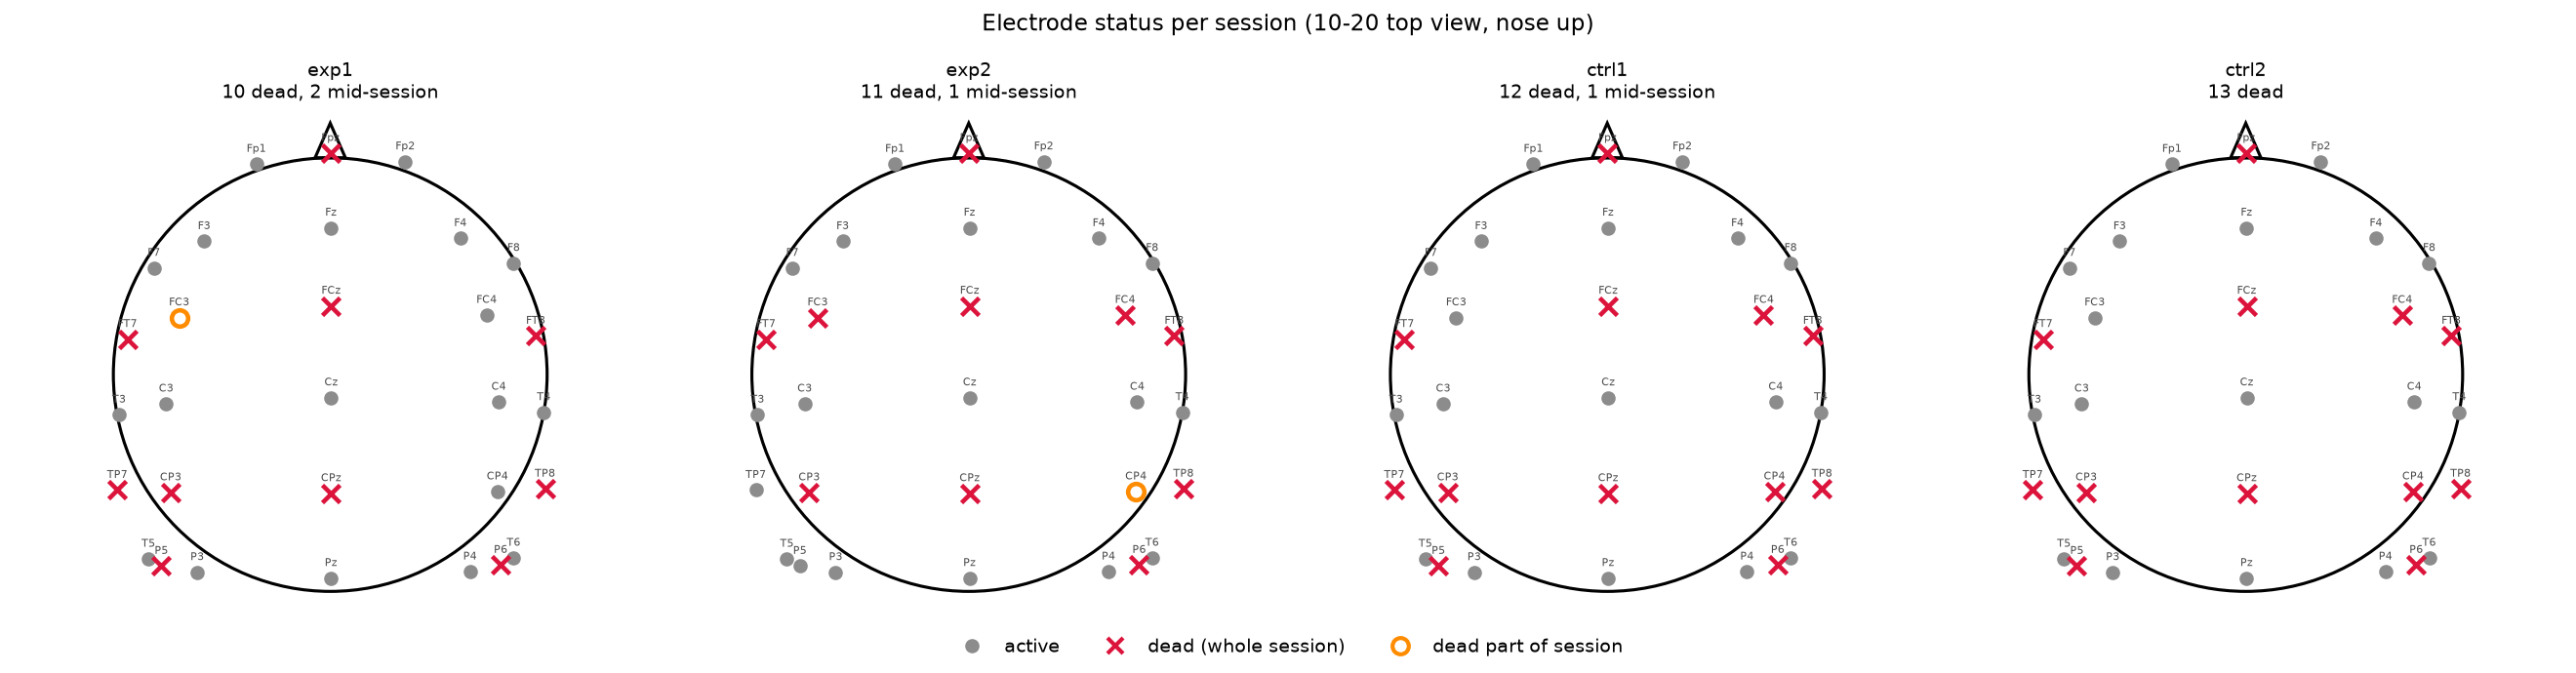
\includegraphics[width=\textwidth]{dead_topomaps.png}
\caption{Статус электродов в каждой сессии (вид сверху, схема размещения 10-20). Одно и то же «кольцо» электродов
(срединные FCz/CPz, латеральные FT7/FT8, TP7/TP8, CP3, P5/P6, Fpz) отключено в каждой сессии и у обоих
испытуемых; оранжевым отмечены каналы, сменившие состояние в процессе записи (FC3 ожил в первый день,
CP4 отвалился во второй, POz «плавал» в части 1 контрольный испытуемый).}
\label{fig:topo}
\end{figure}

\begin{figure}[ht]\centering
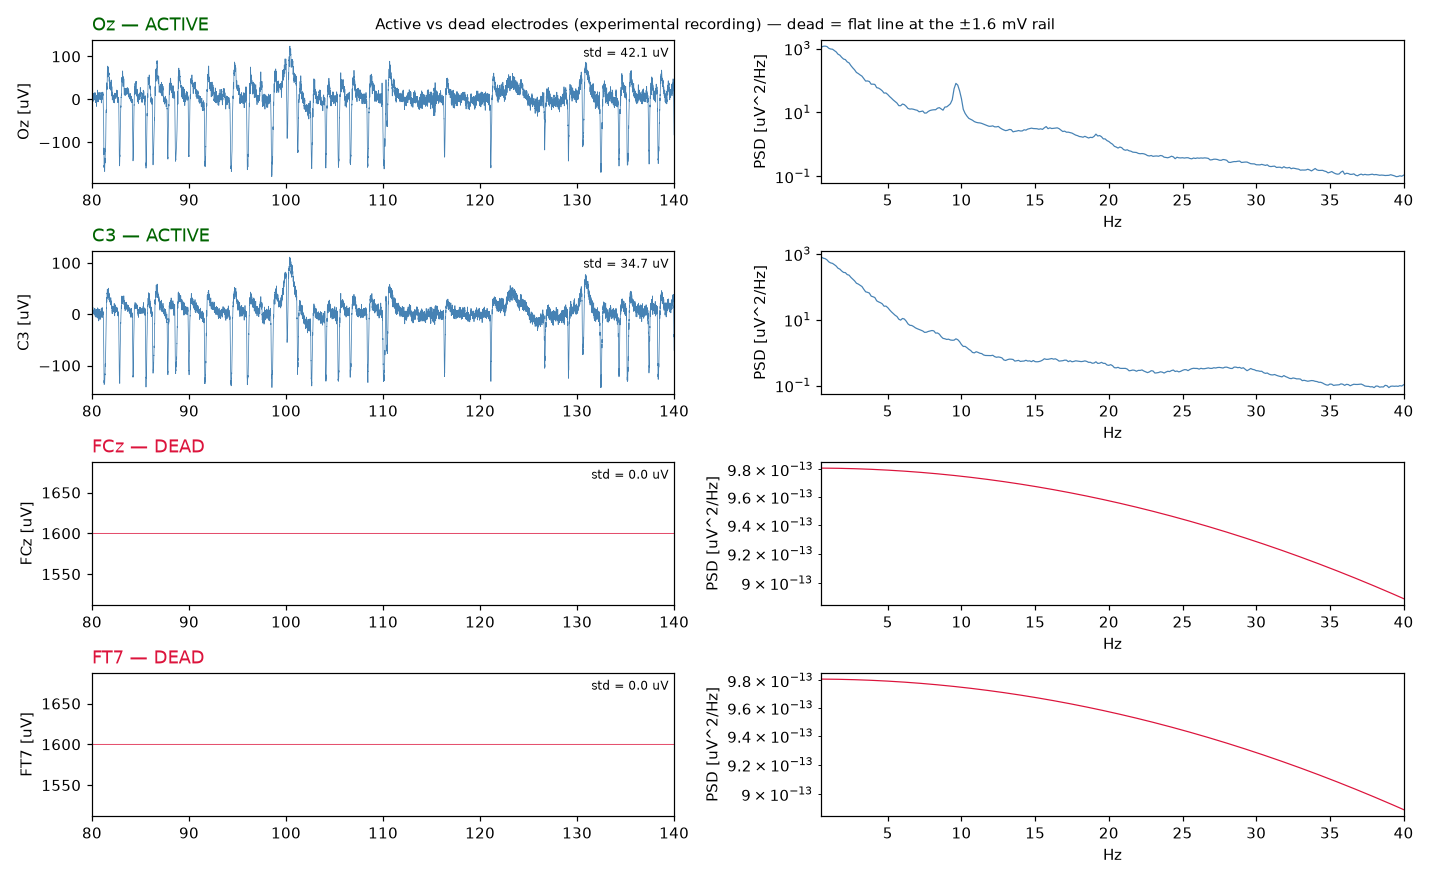
\includegraphics[width=0.95\textwidth]{dead_vs_active.png}
\caption{Активные и мёртвые электроды (испытуемый с заиканием, сессия 1). Активные: реальный сигнал мозга, спектр вида 1/f,
виден альфа-пик. Мёртвые: прямая линия на уровне входа усилителя, нулевое стандартное отклонение,
спектр --- численный шум (на 16 порядков слабее).}
\label{fig:dead}
\end{figure}

Изменения в процессе записи (при анализе нужны списки плохих каналов с учётом времени):
\begin{itemize}\setlength\itemsep{0pt}
\item ИСЗ сессия 1: FC3 \textbf{снова заработал} на $\sim$1050-й секунде (во время чтения); POz
перестал работать на 90-й.
\item ИСЗ сессия 2: CP4 перестал работать на $\sim$1250-й секунде (во время речи).
\item контрольный испытуемый, часть 1: POz «плавал» (работал 0--140 с, мёртв 140--1380 с).
\end{itemize}

\subsection*{2.2 Вспомогательные каналы}
\begin{itemize}\setlength\itemsep{1pt}
\item \textbf{Resp2 в сессии контроля не был подключён} (подтверждено): в обеих частях это чистый шум.
Дыхательный пояс (Pesp) --- настоящий сигнал в обеих частях контрольной записи.
\item \textbf{КГР в части 1 контрольного испытуемого настоящая} --- тот же масштаб амплитуды и тот же фазный рисунок,
что и в части 2 (рис.~\ref{fig:aux}); каналы казались «одинаковыми» только из-за общего пика в момент
аварийного завершения записи.
\item КГР в сессии 2 (ИСЗ) \textbf{очень слабая} (примерно в 10 раз слабее, чем в сессии 1) --- фазные
ответы видны, но датчик был плохо закреплён.
\item Pesp (первый датчик дыхания) мёртв в обеих сессиях (исп. с заиканием).
\end{itemize}

\begin{figure}[ht]\centering
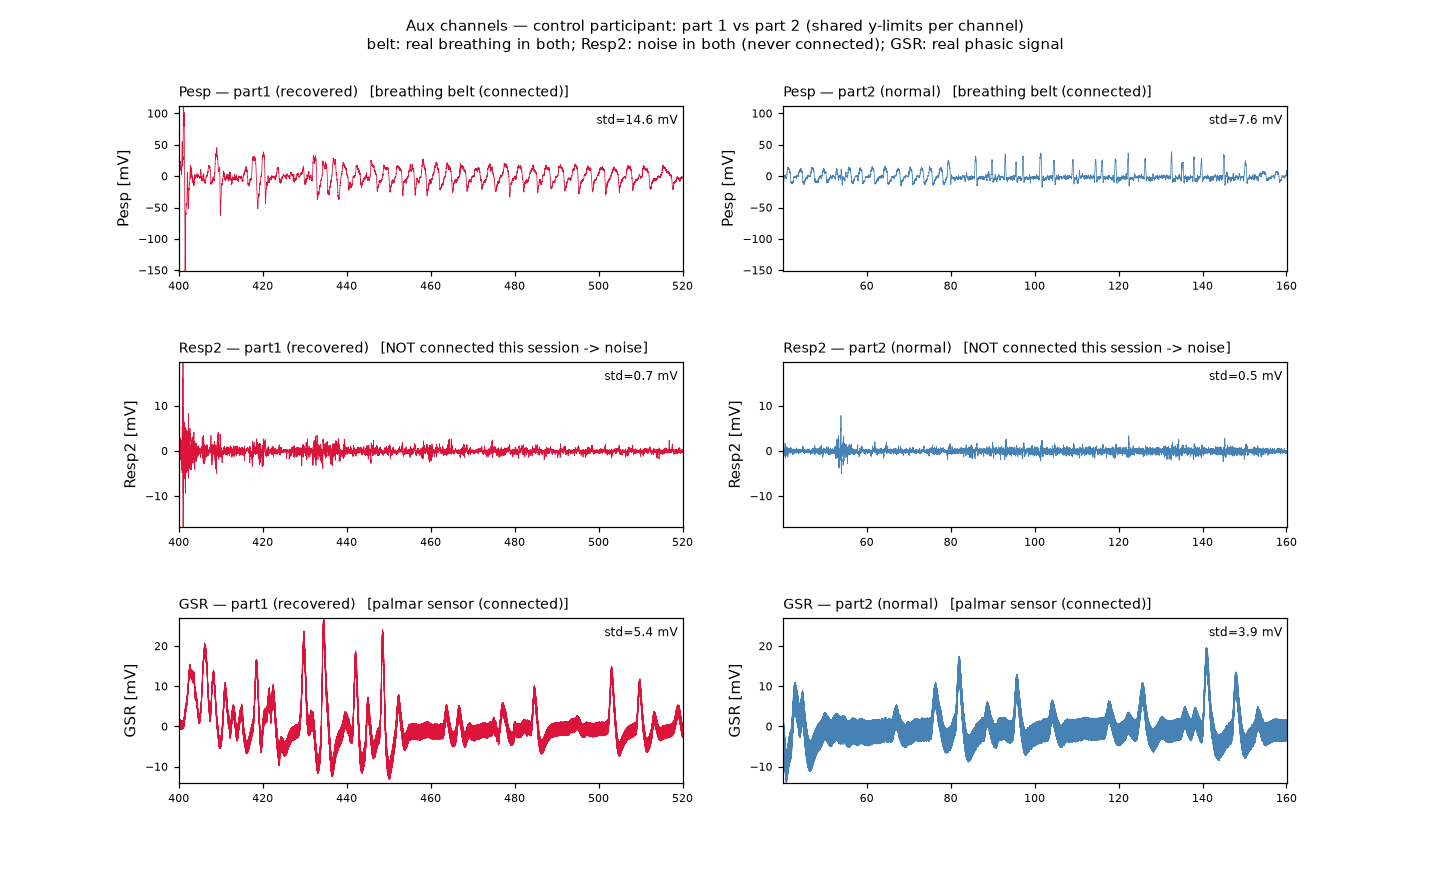
\includegraphics[width=0.95\textwidth]{aux_ctrl_parts.png}
\caption{Вспомогательные каналы контрольного испытуемого: часть 1 (слева) и часть 2 (справа), единый масштаб для каждой
пары. Дыхательный пояс: реальный сигнал в обеих частях. Resp2: шум в обеих (не подключался).
КГР: настоящий фазный сигнал в обеих.}
\label{fig:aux}
\end{figure}

\subsection*{2.3 Метки этапов}
\begin{itemize}\setlength\itemsep{1pt}
\item ИСЗ сессия 1: все 17 меток на месте; каждая фиксированная фаза равна 180,0\,$\pm$\,0,1 с ---
надёжность меток по времени составляет десятки миллисекунд.
\item ИСЗ сессия 2: одна метка отсутствует (\texttt{open\_raw3\_start}); этап восстановлен по интервалу
179,98 с между \texttt{reading\_finish} и \texttt{open\_raw3\_finish} --- ровно одна фаза покоя.
\item контрольный испытуемый, часть 1: \textbf{меток нет вообще}. Причина установлена по «сырому» файлу прибора:
в нём отсутствуют блок событий и финальный блок файла --- метки записываются при штатном закрытии
записи, а сбой ему помешал. Конвертация не виновата (в обычных файлах метки сохраняются).
Вывод: перезапись с начала после сбоя действительно была бы правильным решением. Границы этапов
части 1 оценены по самим данным (окно альфа-ритма с закрытыми глазами и всплеск дыхания соответствуют
порядку протокола); их стоит сверить с видео.
\item Метки «100» --- дублирующие сигналы конца этапа; все стоят в пределах $\leq$1 с после
именованной метки конца этапа, смещения одинаковы в разных сессиях --- могут служить запасными метками.
\end{itemize}

\section*{3. Выглядят ли данные ожидаемо?}
\begin{itemize}\setlength\itemsep{2pt}
\item \textbf{Альфа-ритм в покое: да, образцовый.} Затылочный альфа-ритм (8--12\,Гц) с закрытыми
глазами в 6--20 раз сильнее, чем с открытыми, в каждой записи; чистый пик 10\,Гц появляется в спектре
только с закрытыми глазами (рис.~\ref{fig:psd}). Индивидуальная альфа-частота 9,6--9,9\,Гц,
устойчива между сессиями.
\item \textbf{Моторные артефакты во время речи: да.} Высокочастотная мощность (30--80\,Гц) —
одна из самых высоких среди всех этапов в каждой записи. Записи в целом богаты артефактами
(плохие контакты «двигаются»), поэтому отсеивать артефакты нужно относительными, робастными
методами, а не абсолютными порогами.
\item \textbf{Гипервентиляция: подтверждается наполовину.} \emph{Глубина} дыхания во время
гипервентиляции вырастает в 2--3 раза (амплитуда пояса), но \emph{частота} не увеличивается ни
в одной из трёх записей (13--29/мин и в покое, и при гипервентиляции). Либо дышали глубоко, но
не часто, либо пояс сглаживает быстрые движения. Стоит проверить видео.
\end{itemize}

\begin{figure}[ht]\centering
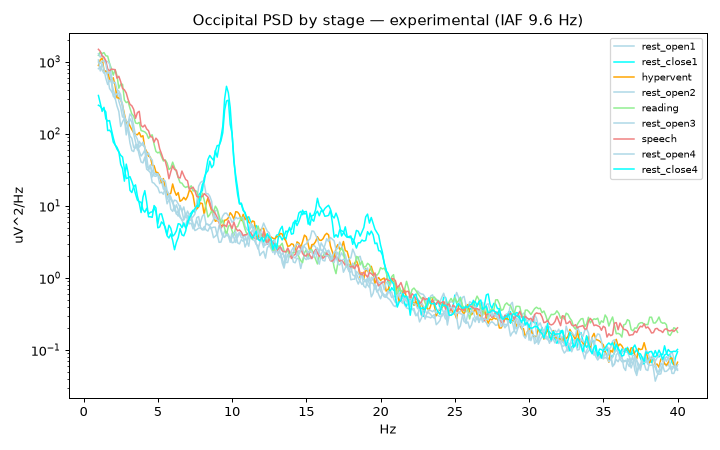
\includegraphics[width=0.49\textwidth]{psd_exp.png}\hfill
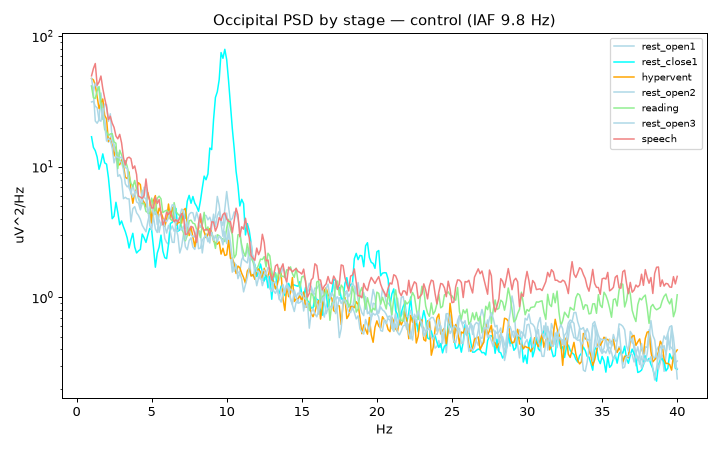
\includegraphics[width=0.49\textwidth]{psd_ctrl.png}
\caption{Затылочные спектры по этапам: кривые с закрытыми глазами (голубые) с доминантным пиком 10\,Гц
у обоих испытуемых; на остальных этапах пика нет.}
\label{fig:psd}
\end{figure}

\section*{4. Исследовательские результаты}

\subsection*{4.1 Реакция на гипервентиляционную пробу (ГВ)}
Каноническая реакция взрослого: «нейрогенное нарастание» тета-медленноволновой активности к концу
гипервентиляции (встречается лишь примерно у трети здоровых взрослых), исчезающее в течение 2 минут
после нормализации дыхания.
\begin{center}\small
\begin{tabular}{@{}llllp{5.6cm}@{}}
\toprule
& тета во время ГВ & конец ГВ & через 3 мин & вердикт \\
\midrule
ИСЗ, день 1 & $+69\%$ & $+98\%$ & всё ещё $+52\%$ & сильное нарастание, \textbf{запаздывающее восстановление} \\
\midrule
ИСЗ, день 2 & $+2\%$ & $+6\%$ & $+19\%$ & \textbf{нарастание отсутствует} \\
\midrule
Контроль & $+29\%$ & $+33\%$ & $+30\%$ & умеренная, типичная реакция \\
\bottomrule
\end{tabular}
\end{center}
\emph{Один и тот же человек} показал противоположные реакции в два дня. Наиболее вероятное объяснение
--- старание/соблюдение инструкции: частота дыхания при гипервентиляции не выросла ни в одной записи,
а реакция второго дня похожа на «работу вполовину». Сохранение медленноволновой активности
более 3 минут в первый день --- единственное «клиническое» наблюдение; физиологически CO$_2$
восстанавливается около 7 минут, так что это может быть вариантом нормы. Высокоамплитудных ритмичных
дельта-эпизодов (тех, что отмечают как клинически значимые) не было ни у кого. КГР во время пробы резко возросла
на $+42\%$ (сессия 1, ИСЗ) --- сильный симпатический ответ. После гипервентиляции альфа-ритм при открытых
глазах повышен \emph{во всех трёх} записях --- либо истинное состояние после пробы, либо привыкание;
разделить их можно, добавив вторую базовую запись перед пробой.

\begin{figure}[ht]\centering
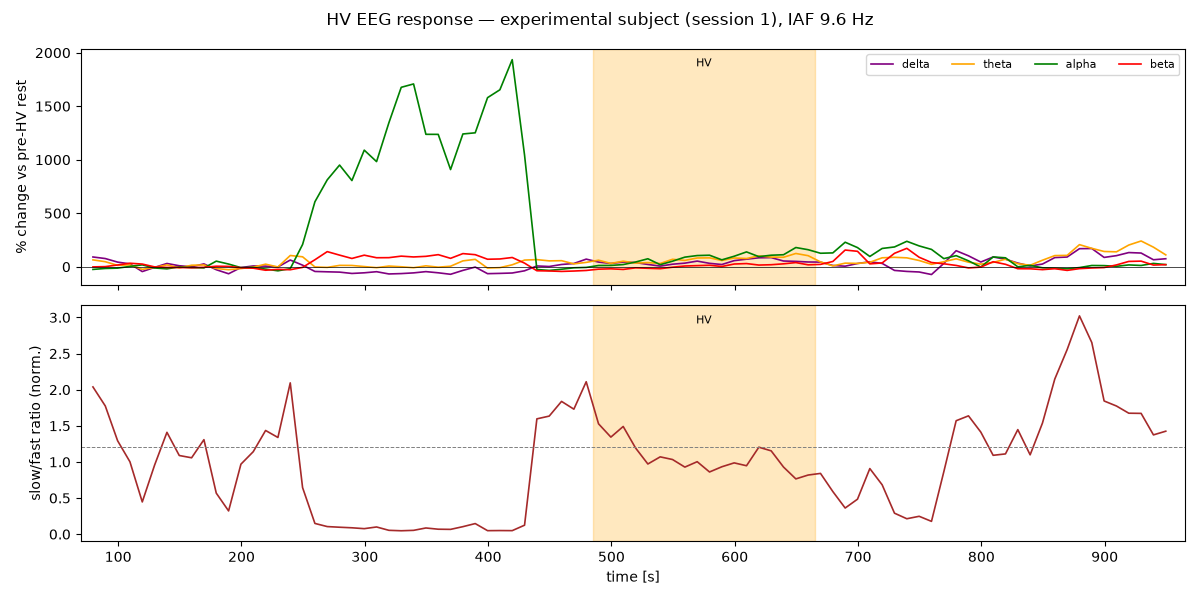
\includegraphics[width=0.9\textwidth]{hv_exp.png}
\caption{Испытуемый с заиканием (сессия 1) вокруг блока гипервентиляции. Вверху: \% изменения
мощности полос относительно покоя с открытыми глазами до пробы; большой зелёный всплеск альфа
до затенённой зоны --- блок с закрытыми глазами. Внизу: соотношение медленная/быстрая остаётся повышенным --- запаздывающее восстановление.}
\end{figure}

\subsection*{4.2 Речь: фронтальный «тета-ритм усилия» различает двух испытуемых}
Фронтально-центральная тета (4--8\,Гц на Fz) --- классический маркер когнитивного контроля и
усилия при обработке. Во время связной речи она выросла на \textbf{+109\% и +69\% у человека
с заиканием (оба дня)} и на \textbf{--4\% у контроля}. Та же картина при чтении вслух
(+79\%/+53\% против +6\%). Это согласуется с литературой по заиканию (повышенная нагрузка
мониторинга/усилия при речи) и воспроизвелось между днями --- самое устойчивое различие между
испытуемыми из найденных. Оговорка: тета чувствительна к морганиям, а испытуемый с заиканием моргает
намного чаще (см. ниже); перед финальными цифрами нужна ICA-очистка.

\subsection*{Слушание и ответ внутри интервью}
Этап речи включает и ответы, и слушание вопросов. Окна были классифицированы без микрофона по
мышечной активности (30--80\,Гц): окна ответа --- всплески мышечной активности, окна слушания ---
тихие паузы между ними (45--50\% неоднозначных окон исключены). Результат уточняет картину:
\begin{center}\small
\begin{tabular}{@{}llll@{}}
\toprule
& фронтальная тета: слушание vs покой & ответ vs слушание & моргания (слуш. $\to$ ответ) \\
\midrule
ИСЗ сессия 1 & $+109\%$ & $+4\%$ & 59 $\to$ 59 /мин \\
ИСЗ сессия 2 & $+71\%$ & $+1\%$ & 61 $\to$ 64 /мин \\
Контроль & $-10\%$ & $+13\%$ & 16 $\to$ 28 /мин \\
\bottomrule
\end{tabular}
\end{center}
У испытуемого с заиканием повышение фронтальной теты \emph{уже максимально во время слушания} ---
это состояние «участия в диалоге», а не артикуляторное усилие само по себе. У контроля обратная,
интуитивная картина: тета около базовой при слушании и умеренный всплеск $+13\%$ при ответе.
Моргания у испытуемого с заиканием высоки в обоих состояниях; у контроля частота морганий
удваивается при речи. Это наблюдение над одним человеком с грубым косвенным разделением на слушание и ответ
(голос интервьюера тоже слышен в окнах «слушания»), но оно меняет главный вывод: маркер различает
\emph{нахождение в диалоге}, а не \emph{говорение}.

\subsection*{Речевые зоны (гомологи Брока и Вернике)}
С электродами 10-20 эти области можно лишь приближённо оценить: зона Брока $\approx$ F7/F3 против
правого гомолога F8/F4; зона Вернике $\approx$ T3/T5 против T4/T6. Сравнение окон интервью
\emph{с покоем} здесь ненадёжно: во время интервью амплитуда \emph{всех} диапазонов (включая
альфа) растёт --- вероятно, пот снижает сопротивление электродов --- поэтому абсолютные изменения
диапазонов неинтерпретируемы. Асимметрия левый/правый \emph{внутри одного состояния} от этой
помехи свободна и информативна (альфа-мощность отражает «простаивание» коры; меньше альфа =
больше активация):
\begin{center}\small
\begin{tabular}{@{}lcccc@{}}
\toprule
альфа L$-$R асимметрия, \% & \multicolumn{2}{c}{гомолог Брока} & \multicolumn{2}{c}{гомолог Вернике} \\
\cmidrule(r){2-3}\cmidrule(l){4-5}
& ответ & слушание & ответ & слушание \\
\midrule
ИСЗ, день 1 & $+27$ & $+27$ & $-15$ & $-15$ \\
ИСЗ, день 2 & $+10$ & $+9$ & $-16$ & $-15$ \\
Контроль & $-4$ & $+2$ & $+19$ & $+1$ \\
Контроль (продолжение) & $+2$ & $+2$ & $+9$ & $+9$ \\
\bottomrule
\end{tabular}
\end{center}
У испытуемого с заиканием в оба дня устойчивая картина: \textbf{относительное «простаивание» левого
гомолога зоны Брока} (положительное = больше левой альфа = меньше левая активация, от $+10$ до
$+27\%$) и \textbf{правосторонний гомолог зоны Вернике} ($-15\%$), т.\,е.\ смещение латерализации
вправо при речевой деятельности --- направление согласуется с литературой по заиканию
(гипоактивация левых лобных/задневисочных отделов с подключением правого полушария). У контроля
баланс или левосторонний уклон. Две оговорки: (1) асимметрия одинакова при ответе и при слушании
--- снова тоническое «речевое» состояние, а не эффект, вызванный говорением; (2) T3--T6 расположены
над височной мышцей, поэтому цифры по зоне Вернике --- более слабые. Окончательные ответы
потребуют локализации уровня фМРТ или хотя бы высокоплотной шапочки.

\subsection*{Чтение вслух против диалога: усилие то же, а запинок --- по-разному}
Наблюдение: при чтении вслух у испытуемого с заиканием запинки были заметны, тогда как в диалоге
запинок практически не было --- в противоположность классическому «облегчающему» эффекту чтения
из литературы.
Прямое сравнение двух вокальных задач (от интервью взяты только окна речи, чтобы обе задачи были
произнесением) даёт содержательный отрицательный результат:
\begin{center}\small
\begin{tabular}{@{}lcccc@{}}
\toprule
& фронтальная тета & альфа & моргания & Брока L$-$R \\
\midrule
ИСЗ сессия 1: чтение $\to$ ответ & $+3\%$ & $+10\%$ & 46$\to$60/мин & $+19\to+27\%$ \\
ИСЗ сессия 2: чтение $\to$ ответ & $+7\%$ & $+20\%$ & 46$\to$63/мин & $0\to+10\%$ \\
Контроль: чтение $\to$ ответ & $-1\%$ & (завышено мышцами) & 16$\to$23/мин & $-4\to-4\%$ \\
\bottomrule
\end{tabular}
\end{center}
У испытуемого с заиканием картина «коркового усилия» практически \emph{одинакова} в двух вокальных
задачах (фронтальная тета 14.1 против 14.5 и 11.2 против 12.0\,$\mu$V$^2$; тоническая КГР 278 против
294\,мВ, частота фазных ответов КГР (SCR, skin conductance response) 13.8 против 11.0/мин) --- хотя запинок в этих задачах было разное количество. Значит, повышенная
тета \emph{не} отслеживает запинки; она маркирует состояние произнесения «под наблюдением».
Разница в количестве запинок между чтением и диалогом должна находиться на уровне речемоторного
планирования,
которое скальповая ЭЭГ с 36 каналами не разрешает --- и которое здесь не ловит ни один
частотный контраст. Полноценный анализ запинок требует аудио (отсутствует) плюс размеченные по
видео события запинок, привязанные к ЭЭГ: это то единственное, что мы бы в первую очередь
посоветовали добавить в протокол в следующий раз.

\subsection*{4.3 Возбуждение: частота морганий и КГР}
\begin{itemize}\setlength\itemsep{1pt}
\item Частота морганий в покое: \textbf{30--52/мин у испытуемого с заиканием против 4--16/мин
у контроля} (в 2--4 раза); во время речи растёт на $\sim$35\% у обоих. Согласуется с повышенным
тоническим возбуждением/тревогой; корректно как внутрииндивидуальное сравнение.
\item Тоническая КГР в сессии 1 (ИСЗ) растёт на протяжении всей сессии (187 $\rightarrow$ 294\,мВ от первого
покоя до речи) и после речи снижается лишь частично --- возбуждение накапливается по ходу протокола.
\end{itemize}

\subsection*{4.4 «Гипоксические» эффекты после речи: не обнаружены}
В 3-минутном покое после речи нет ни замедления, ни снижения альфа-ритма относительно покоя перед
речью (изменения $\leq$1\%) ни в одной записи. Эффекты речи здесь --- возбуждение и усилие, и они
проходят в течение нескольких минут. («Гипоксический» ЭЭГ-рисунок относится к гипервентиляции из-за падения
CO$_2$, а не к речи.)

\subsection*{4.5 Другие аномалии ЭЭГ --- результаты скрининга}
\begin{itemize}\setlength\itemsep{1pt}
\item \textbf{Активности, похожей на эпилептиформную, нет.} Автоматический скрининг пиков/острых волн
плюс визуальный просмотр главных кандидатов нашли только артефакты морганий (фронтальные медленные
отклонения) и мышечные залпы (рис.~\ref{fig:spikes}).
\item \textbf{Очаговых ритмичных дельта-эпизодов} нигде нет.
\item \textbf{Помехи 50\,Гц отсутствуют}; проблем с постоянной составляющей и насыщением нет,
кроме известных мёртвых электродов.
\item \textbf{Одно наблюдение:} у испытуемого с заиканием альфа-ритм с закрытыми глазами заметно
правосторонний по задним отведениям (теменные P3/P4: от --54 до --68\%, затылочные: от --23 до --35\%),
и рисунок \emph{повторяется в оба дня}; у контроля асимметрии малы и неустойчивы. Это может быть
как физиологией (асимметрия альфа-ритма), так и артефактом контакта --- проверить сопротивление
P3/P4/O1/O2 прежде, чем интерпретировать.
\end{itemize}

\begin{figure}[ht]\centering
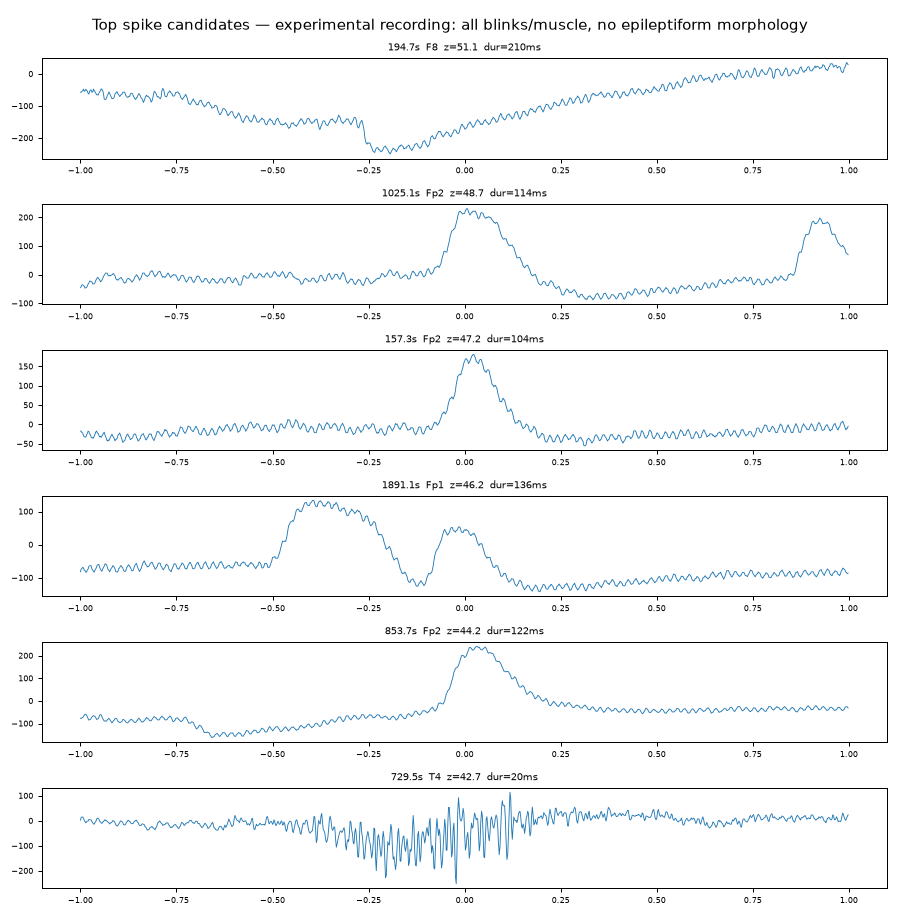
\includegraphics[width=0.9\textwidth]{spike_candidates.png}
\caption{Лучшие автоматические кандидаты в «пики» (испытуемый с заиканием, сессия 1): все --- моргания (Fp1/Fp2, медленные
положительные отклонения) или мышечные залпы (T4); эпилептиформной морфологии нет.}
\label{fig:spikes}
\end{figure}

\section*{5. Выводы и рекомендации}
\begin{enumerate}\setlength\itemsep{1pt}
\item Все четыре записи пригодны для анализа: ИСЗ сессия 1 --- полностью; ИСЗ сессия 2 --- со слабой КГР и
одним восстановленным этапом; контрольный испытуемый часть 1 --- с оценочными границами этапов (сверить с видео)
и без Resp2; часть 2 --- полностью.
\item Оборудование: кольцо мёртвых электродов одинаково во всех сессиях и у обоих испытуемых
$\rightarrow$ проверить электроды/гнёзда разъёма; выяснить, почему проверка сопротивления «пропускает»
примерно треть неподключённых электродов.
\item Протокол: контролировать соблюдение инструкции при гипервентиляции (видео; в идеале EtCO$_2$);
добавить вторую базовую запись перед пробой; после сбоя всегда перезаписывать с начала (метки части 1
не восстановимы).
\item Анализ: списки плохих каналов с учётом времени; робастное относительное отсеивание артефактов;
ICA/CleanLine перед количественной оценкой фронтальной теты и морганий.
\item Исследовательские зацепки для расширения выборки: устойчивое повышение фронтальной теты на
всём протяжении интервью (одинаково при слушании и ответе) у испытуемого с заиканием,
воспроизведённое в оба дня, в отличие от специфичного для речи всплеска теты у контроля;
повышенная частота морганий в покое;
запаздывающее восстановление после гипервентиляции; правосторонняя асимметрия заднего альфа-ритма
(после исключения проблем с контактами).
\end{enumerate}

\end{document}
